% tugas_data_analitik.tex
% Laporan Tugas Data Analitik — C-MAPSS FD001 RUL Prediction
% Departemen Teknik Mesin FTUI — 2026

\documentclass[11pt,a4paper]{article}

\usepackage[T1]{fontenc}
\usepackage[utf8]{inputenc}
\usepackage[a4paper, margin=2.5cm]{geometry}
\usepackage{setspace}
\usepackage{parskip}
\usepackage{titlesec}
\usepackage{fancyhdr}
\usepackage{booktabs}
\usepackage{tabularx}
\usepackage{multirow}
\usepackage{graphicx}
\usepackage{caption}
\usepackage{subcaption}
\usepackage{xcolor}
\usepackage{amsmath}
\usepackage{amssymb}
\usepackage{hyperref}
\usepackage{enumitem}
\usepackage{float}
\usepackage{tocloft}
\usepackage{url}

\definecolor{uiblue}{RGB}{0,56,147}
\definecolor{mygray}{RGB}{100,100,100}

\titleformat{\section}
  {\large\bfseries\color{uiblue}}
  {\thesection}{0.6em}{}[\vspace{2pt}\hrule\vspace{4pt}]
\titleformat{\subsection}
  {\normalsize\bfseries\color{uiblue}}{\thesubsection}{0.6em}{}
\titleformat{\subsubsection}
  {\small\bfseries}{\thesubsubsection}{0.6em}{}

\pagestyle{fancy}
\fancyhf{}
\fancyhead[L]{\small\color{mygray}
  Tugas Data Analitik -- Prediksi RUL Mesin Turbofan C-MAPSS FD001}
\fancyhead[R]{\small\color{mygray} Data Analitik 2026}
\fancyfoot[C]{\small\color{mygray}\thepage}
\renewcommand{\headrulewidth}{0.4pt}
\renewcommand{\footrulewidth}{0.0pt}

\onehalfspacing
\captionsetup{font=small, labelfont=bf}
\hypersetup{colorlinks=true, linkcolor=uiblue,
            urlcolor=uiblue, citecolor=uiblue}

% ══════════════════════════════════════════════════════════════════════════════
\begin{document}

% ── Cover ─────────────────────────────────────────────────────────────────────
\begin{titlepage}
  \centering
  \vspace*{1.0cm}
  
\includegraphics[width=2.2cm]{images/logo_ui.png}
  \vspace{0.6cm}

  {\large\bfseries UNIVERSITAS INDONESIA\par}
  \vspace{0.2cm}
  {\normalsize Fakultas Teknik -- Departemen Teknik Mesin\par}

  \vspace{0.5cm}
  \hrule height 1.2pt
  \vspace{0.4cm}
  {\LARGE\bfseries\color{uiblue}
    PREDIKSI \textit{REMAINING USEFUL LIFE}\\[0.3em]
    MESIN TURBOFAN MENGGUNAKAN\\[0.3em]
    \textit{ARTIFICIAL NEURAL NETWORK}\\[0.3em]
    PADA DATASET C-MAPSS FD001\par}
  \vspace{0.4cm}
  \hrule height 1.2pt

  \vspace{1.0cm}
  {\normalsize\color{mygray} Mata Kuliah:\par}
  {\large\bfseries Data Analitik\par}
  \vspace{0.6cm}
  {\normalsize\color{mygray} Dosen Pengampu:\par}
  {\normalsize Dr.\ Eng.\ Sholahudin, S.T., M.Sc.\par}

  \vspace{0.8cm}
  {\normalsize\color{mygray} Disusun Oleh:\par}
  \vspace{0.4cm}
  \begin{tabular}{ll}
    2506565466 & Luqman Alifio Arhab \\[4pt]
    2506565414 & Azfa Rhazasta Abiandra \\[4pt]
    2506565401 & Adamsyah Haryo Saksono \\[4pt]
    2506565433 & Epsiarto Rizqi Nurwijayadi \\[4pt]
  \end{tabular}

  \vspace{0.2cm}
  \vfill
  {\normalsize\bfseries
    DEPARTEMEN TEKNIK MESIN\\
    FAKULTAS TEKNIK\\
    UNIVERSITAS INDONESIA\\[0.4em]
    2026\par}
\end{titlepage}

\thispagestyle{empty}
\newpage
\setcounter{page}{1}
\tableofcontents
\newpage

% ══════════════════════════════════════════════════════════════════════════════
\section{Pendahuluan}

\subsection{Latar Belakang}

Prediksi \textit{Remaining Useful Life} (RUL) merupakan komponen kunci dalam
sistem \textit{Prognostics and Health Management} (PHM). Dengan mengetahui
sisa umur pakai komponen sebelum kegagalan, jadwal perawatan dapat dioptimalkan
sehingga mengurangi biaya \textit{downtime} tak terencana dan risiko kegagalan
mendadak.

\begin{figure}[H]
  \centering
  
\includegraphics[width=0.58\textwidth]{images/01_phm_ecosystem_stack.png}
  \caption{Hierarki PHM --- laporan ini berfokus pada lapisan
    \textit{Prognostics} (prediksi RUL)}
  \label{fig:phm}
\end{figure}

Pada mesin turbofan penerbangan, degradasi komponen seperti
\textit{High Pressure Compressor} (HPC) berlangsung secara gradual dan
tercermin dalam perubahan pola sensor. Laporan ini menggunakan sub-dataset
\textbf{FD001} dari C-MAPSS NASA: satu kondisi operasi, satu mode kerusakan
(HPC), 100 mesin \textit{train}, 100 mesin \textit{test}.

\subsection{Tujuan}

\begin{enumerate}[noitemsep]
  \item Membersihkan data dengan analisis korelasi sensor terhadap output (RUL)
  \item Menormalisasi data dengan metode \textit{z-score} berbasis siklus sehat
  \item Memilih fitur menggunakan korelasi Pearson dan PCA
  \item Membangun model MLP untuk prediksi RUL
  \item Menganalisis kepentingan fitur dengan algoritma Garson
\end{enumerate}

\subsection{Alur Pipeline}

\begin{figure}[H]
  \centering\small
  \begin{tabular}{ccccc}
    \fbox{Raw .txt} & $\rightarrow$ &
    \fbox{HDF5} & $\rightarrow$ &
    \fbox{Cleaning} \\[6pt]
    & & & & $\downarrow$ \\[2pt]
    \fbox{Garson} & $\leftarrow$ &
    \fbox{ANN} & $\leftarrow$ &
    \fbox{Normalisasi + PCA}
  \end{tabular}
  \caption{Alur pipeline analitik}
  \label{fig:pipeline}
\end{figure}

% ══════════════════════════════════════════════════════════════════════════════
\section{Dataset C-MAPSS FD001}

\subsection{Deskripsi}

Dataset C-MAPSS dipublikasikan oleh NASA \cite{saxena2008} dan dapat diunduh
dari repositori NASA PCoE:
\begin{center}
  \small\url{https://www.nasa.gov/intelligent-systems-division/discovery-and-systems-health/pcoe/pcoe-data-set-repository/}
\end{center}

\begin{figure}[H]
  \centering
  
\includegraphics[width=0.85\textwidth]{images/09_dataset_matrix.png}
  \caption{Matriks karakteristik empat sub-dataset C-MAPSS ---
    laporan ini menggunakan \textbf{FD001} (termudah: 1 kondisi, 1 mode kerusakan)}
  \label{fig:dataset_matrix}
\end{figure}

FD001 terdiri dari 20.631 baris data \textit{train} (100 mesin, siklus penuh
hingga kegagalan) dan 13.096 baris \textit{test} (100 mesin, dipotong sebelum
kegagalan). File \texttt{RUL\_FD001.txt} berisi 100 nilai RUL sebenarnya
pada titik pemotongan sebagai kunci jawaban evaluasi.

\subsection{Struktur Mesin dan Sensor}

\begin{figure}[H]
  \centering
  
\includegraphics[width=0.88\textwidth]{images/03_cmapss_engine_schematic.png}
  \caption{Skema mesin turbofan C-MAPSS --- 21 sensor mengukur kondisi
    di sepanjang aliran udara; HPC adalah komponen yang mengalami degradasi}
  \label{fig:engine}
\end{figure}

Setiap baris data terdiri dari 26 kolom: \texttt{unit\_number},
\texttt{time\_cycles}, tiga \textit{op\_settings}, dan 21 sensor.

\subsection{Konsep RUL dan File Data}

\begin{figure}[H]
  \centering
  
\includegraphics[width=0.85\textwidth]{images/10_train_test_rul_relationship.png}
  \caption{Hubungan antara file train, test, dan RUL ---
    data \textit{test} dipotong di siklus $t^*$;
    \texttt{RUL\_FD001.txt} berisi siklus tersisa setelah $t^*$}
  \label{fig:rul_rel}
\end{figure}

\subsection{Struktur HDF5}

Seluruh data disimpan dalam \texttt{cmapss\_FD001.h5} menggunakan satu skrip
\texttt{build\_cmapss\_complete.py} yang membaca langsung dari file \texttt{.txt}
NASA tanpa file perantara.

\begin{figure}[H]
  \centering
  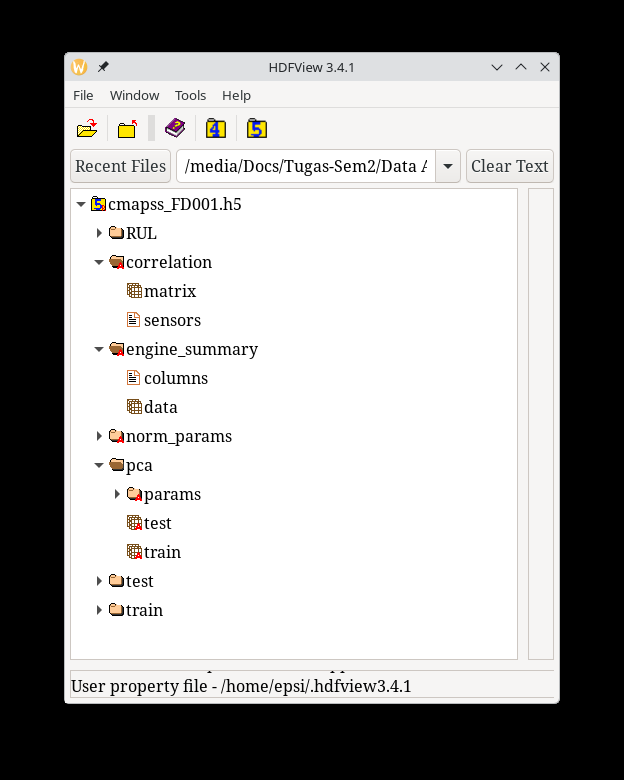
\includegraphics[width=0.38\textwidth]{images/hdf5-05-pca-01-main.png}
  \caption{Struktur HDF5 lengkap \texttt{cmapss\_FD001.h5} di HDFView}
  \label{fig:hdf5}
\end{figure}

% ══════════════════════════════════════════════════════════════════════════════
\section{Pembersihan Data}

\subsection{Metode}

Pembersihan data dilakukan dengan menganalisis korelasi setiap sensor terhadap
output (RUL). Sensor yang tidak membawa informasi degradasi dieliminasi
menggunakan lima metode statistik:

\begin{enumerate}[noitemsep]
  \item \textbf{Standar Deviasi} --- sensor konstan (std $= 0$) tidak bervariasi
  \item \textbf{Koefisien Variasi (CV)} --- $\text{CV} = \sigma/|\mu|$;
    nilai sangat kecil menunjukkan variasi tidak signifikan
  \item \textbf{Korelasi Pearson vs RUL} --- hubungan linear sensor terhadap output
  \item \textbf{Korelasi Spearman vs RUL} --- hubungan monoton sensor terhadap output
  \item \textbf{Mutual Information vs RUL} --- hubungan non-linear sensor terhadap output
\end{enumerate}

\subsection{Hasil Analisis FD001}

\begin{table}[H]
\centering\small
\caption{Statistik sensor FD001 terhadap output RUL ---
  sensor dengan std $= 0$ ditandai ($\dagger$)}
\label{tab:sensor_stats}
\begin{tabular}{lrrrrrrl}
\toprule
Sensor & Mean & Std & CV & Pearson & Spearman & MI & Hapus \\
\midrule
T2$^\dagger$         & 518.67 & 0.000 & 0.000 & NaN     & NaN     & 0.000 & \checkmark \\
T24          & 642.68 & 0.500 & 0.001 & $-$0.607 & $-$0.629 & 0.342 & \\
T30          & 1590.5 & 6.131 & 0.004 & $-$0.585 & $-$0.606 & 0.306 & \\
T50          & 1408.9 & 9.001 & 0.006 & $-$0.679 & $-$0.702 & 0.467 & \\
P2$^\dagger$         &  14.62 & 0.000 & 0.000 & NaN     & NaN     & 0.006 & \checkmark \\
P15          &  21.61 & 0.001 & 0.000 & $-$0.128 & $-$0.128 & 0.006 & \checkmark \\
P30          & 553.37 & 0.885 & 0.002 & $+$0.657 & $+$0.679 & 0.425 & \\
Nf           & 2388.1 & 0.071 & 0.000 & $-$0.564 & $-$0.574 & 0.258 & \\
Nc           & 9065.2 & 22.08 & 0.002 & $-$0.390 & $-$0.322 & 0.222 & \\
epr$^\dagger$        &   1.30 & 0.000 & 0.000 & NaN     & NaN     & 0.000 & \checkmark \\
Ps30         &  47.54 & 0.267 & 0.006 & $-$0.696 & $-$0.718 & 0.507 & \\
phi          & 521.41 & 0.738 & 0.001 & $+$0.672 & $+$0.693 & 0.442 & \\
NRf          & 2388.1 & 0.072 & 0.000 & $-$0.563 & $-$0.573 & 0.262 & \\
NRc          & 8143.8 & 19.08 & 0.002 & $-$0.307 & $-$0.202 & 0.225 & \\
BPR          &   8.44 & 0.038 & 0.004 & $-$0.643 & $-$0.666 & 0.390 & \\
farB$^\dagger$       &   0.03 & 0.000 & 0.000 & NaN     & NaN     & 0.000 & \checkmark \\
htBleed      & 393.21 & 1.549 & 0.004 & $-$0.606 & $-$0.629 & 0.328 & \\
Nf\_dmd$^\dagger$    & 2388.0 & 0.000 & 0.000 & NaN     & NaN     & 0.000 & \checkmark \\
PCNfR\_dmd$^\dagger$ & 100.00 & 0.000 & 0.000 & NaN     & NaN     & 0.000 & \checkmark \\
W31          &  38.82 & 0.181 & 0.005 & $+$0.629 & $+$0.653 & 0.367 & \\
W32          &  23.29 & 0.108 & 0.005 & $+$0.636 & $+$0.657 & 0.380 & \\
\bottomrule
\multicolumn{8}{l}{\small $^\dagger$ std $= 0$: Pearson/Spearman tidak terdefinisi (NaN);
  tidak ada korelasi dengan RUL}
\end{tabular}
\end{table}

Enam sensor dengan std $= 0$ dieliminasi:
\textbf{T2, P2, epr, farB, Nf\_dmd, PCNfR\_dmd}.
Sensor P15 juga dieliminasi karena CV $\approx 0$ dan Pearson $= -0{,}13$
(hampir tidak ada korelasi dengan RUL).
Tersisa \textbf{15 sensor} aktif untuk normalisasi dan pemodelan.

% ══════════════════════════════════════════════════════════════════════════════
\section{Normalisasi}

\subsection{Metode Z-Score Berbasis Siklus Sehat}

\begin{figure}[H]
  \centering
  
\includegraphics[width=0.80\textwidth]{images/13_normalization_pipeline.png}
  \caption{Pipeline normalisasi --- parameter dihitung dari siklus sehat
    (RUL\_raw $\geq 125$), diterapkan ke seluruh data}
  \label{fig:norm_pipeline}
\end{figure}

Normalisasi menggunakan formula \textit{z-score}:
\begin{equation}
  z = \frac{x - \mu_{\text{healthy}}}{\sigma_{\text{healthy}}}
  \label{eq:zscore}
\end{equation}

di mana $\mu$ dan $\sigma$ dihitung hanya dari siklus dengan
RUL\_raw $\geq 125$ (\textit{healthy cycles}).

\subsection{Alasan Penggunaan Siklus Sehat}

Jika parameter dihitung dari seluruh siklus termasuk yang terdegradasi,
nilai $z = 0$ tidak lagi merepresentasikan kondisi sehat. Dengan menggunakan
siklus sehat sebagai referensi: siklus sehat menghasilkan $z \approx 0$,
sedangkan siklus terdegradasi menyimpang dari 0 --- penyimpangan inilah yang
dipelajari model ANN.

\subsection{Penerapan ke Data Test}

Data \textit{test} dinormalisasi menggunakan parameter dari data \textit{train}:
\begin{equation}
  z_{\text{test}} =
  \frac{x_{\text{test}} - \mu_{\text{train, healthy}}}
       {\sigma_{\text{train, healthy}}}
\end{equation}

Menggunakan parameter \textit{test} sendiri merupakan \textit{data leakage}
karena distribusi data masa depan tidak diketahui saat \textit{deployment}.

% ══════════════════════════════════════════════════════════════════════════════
\section{Seleksi Fitur}

\subsection{Korelasi Pearson Antar Sensor}

Matriks korelasi Pearson dihitung dari \texttt{train\_normalized} untuk
mengidentifikasi redundansi antar sensor.

\begin{figure}[H]
  \centering
  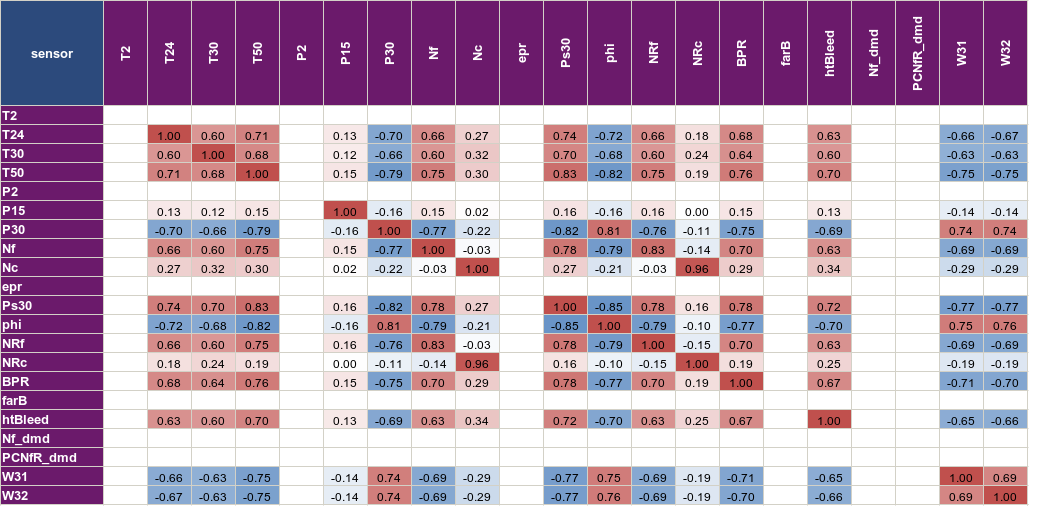
\includegraphics[width=0.80\textwidth]{images/spreadsheet-05-correlation-05-correlations.png}
  \caption{Matriks korelasi Pearson antar sensor (FD001) ---
    merah = korelasi positif kuat, biru = negatif kuat}
  \label{fig:corr}
\end{figure}

Pasangan Nf--NRf ($r = 0{,}83$) dan Nc--NRc ($r = 0{,}96$) menunjukkan
redundansi tinggi --- motivasi utama penggunaan PCA untuk mereduksi dimensi.

\subsection{Principal Component Analysis (PCA)}

\subsubsection{Varians yang Dijelaskan}

PCA diterapkan pada 15 sensor ternormalisasi. Tabel berikut menunjukkan
varians individual per komponen:

\begin{table}[H]
\centering\small
\caption{Varians PCA FD001 (15 sensor $\to$ 15 komponen)}
\label{tab:pca_var}
\begin{tabular}{lrrrrrrrr}
\toprule
& PC1 & PC2 & PC3 & PC4 & PC5 & PC6 & PC7 & PC8 \\
\midrule
Individual & 52,4\% & 30,5\% & 2,0\% & 1,8\% & 1,7\% & 1,6\% & 1,6\% & 1,4\% \\
Kumulatif  & 52,4\% & 82,9\% & 84,9\% & 86,7\% & 88,4\% & 90,1\% & 91,7\% & 93,0\% \\
\bottomrule
\end{tabular}
\end{table}

Terdapat \textit{scree cliff} setelah PC2: PC1 = 52,4\% dan PC2 = 30,5\%,
kemudian PC3 hanya 2,0\%. PC1 dan PC2 bersama-sama menjelaskan \textbf{82,9\%}
varians data.

\subsubsection{Pemilihan Komponen}

Kriteria \textbf{Opsi B}: pertahankan komponen dengan varians individual
$\geq 5\%$. Hasilnya: \textbf{2 komponen} dipertahankan (PC1 dan PC2).

\subsubsection{Interpretasi Eigenvectors}

\begin{figure}[H]
  \centering
  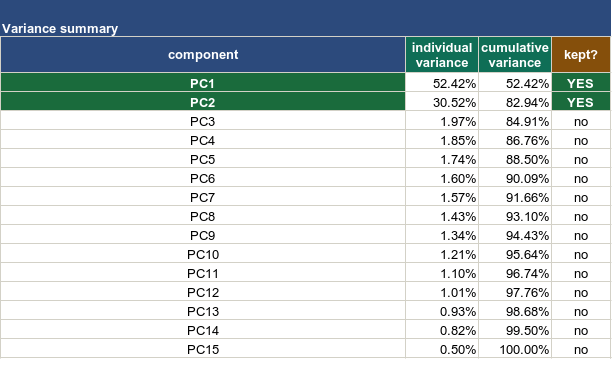
\includegraphics[width=0.80\textwidth]{images/spreadsheet-06-pca-11a-pca-params.png}
  \caption{Tabel varians dan matriks \textit{eigenvectors} FD001 di spreadsheet v6}
  \label{fig:pca_params}
\end{figure}

\begin{itemize}[noitemsep]
  \item \textbf{PC1} (52,4\%): didominasi Nf, NRf, Nc, NRc ---
    merepresentasikan \textit{overall engine speed state}
  \item \textbf{PC2} (30,5\%): kontras antara sensor kecepatan dan sensor
    tekanan/suhu --- merepresentasikan \textit{compressor loading condition}
\end{itemize}

\subsection{Pipeline Spreadsheet}

Seluruh analisis juga didokumentasikan dalam spreadsheet v1--v6:

\begin{table}[H]
\centering\small
\caption{Evolusi spreadsheet v1--v6}
\label{tab:spreadsheet}
\begin{tabular}{llp{9cm}}
\toprule
Versi & Sheet Baru & Isi \\
\midrule
v3 & train, test, RUL & Data raw + kolom komputasi (condition\_id, dT, RUL) \\
v4 & train\_normalized  & Sensor ternormalisasi \\
v5 & test\_normalized, stats, correlation, engine\_summary
   & Normalisasi test, statistik, korelasi, ringkasan mesin \\
v6 & pca\_params, pca\_train, pca\_test & Parameter PCA + skor PC per siklus \\
\bottomrule
\end{tabular}
\end{table}

\begin{figure}[H]
  \centering
  \begin{subfigure}[b]{0.48\textwidth}
    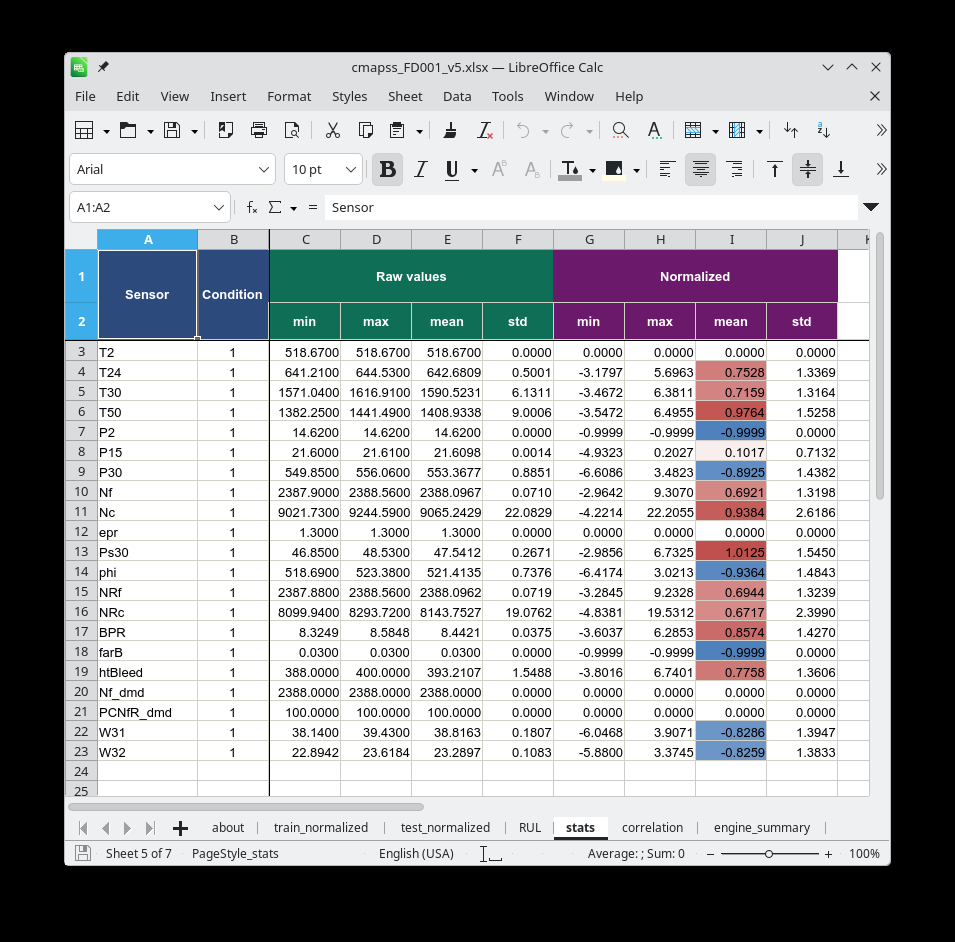
\includegraphics[width=\textwidth]{images/workbook-05-correlation-04-statistics.png}
    \caption{Sheet \texttt{stats} (v5)}
  \end{subfigure}
  \hfill
  \begin{subfigure}[b]{0.48\textwidth}
    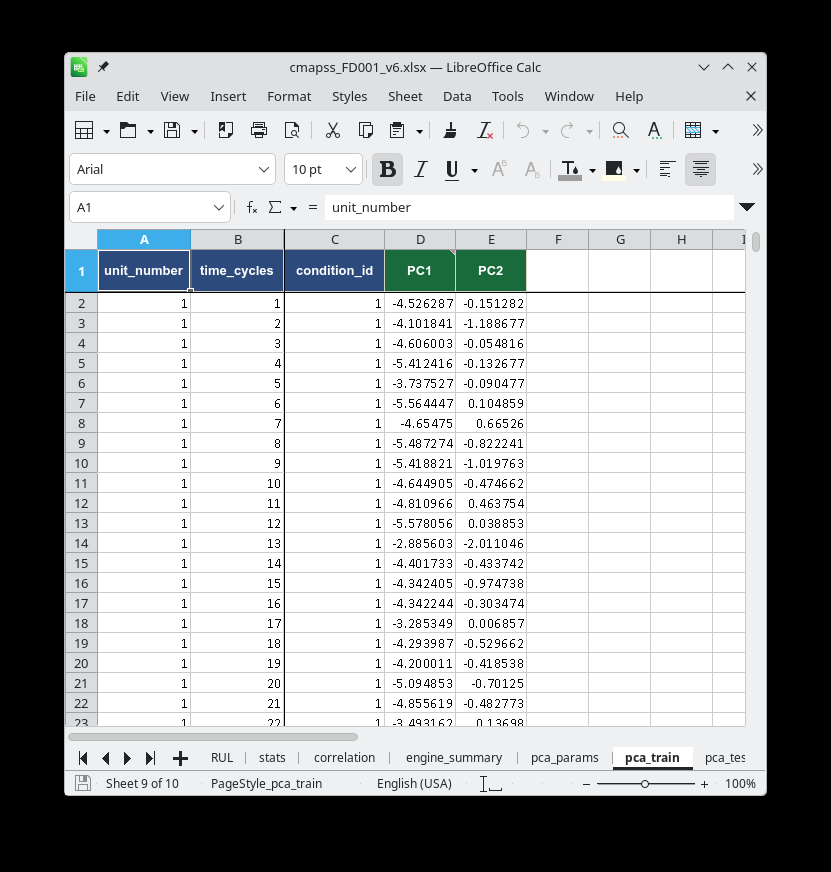
\includegraphics[width=\textwidth]{images/workbook-06-pca-12-pca-train.png}
    \caption{Sheet \texttt{pca\_train} (v6)}
  \end{subfigure}
  \caption{Contoh sheet spreadsheet v5 dan v6}
  \label{fig:spreadsheet}
\end{figure}

% ══════════════════════════════════════════════════════════════════════════════
\section{Model \textit{Artificial Neural Network}}

\subsection{Arsitektur dan Konfigurasi}

Model \textit{Multilayer Perceptron} (MLP):
\begin{equation}
  \text{input} \xrightarrow{W_1,\,\text{ReLU}}
  64 \xrightarrow{W_2,\,\text{ReLU}}
  32 \xrightarrow{W_3}
  1
\end{equation}

\begin{table}[H]
\centering\small
\caption{Konfigurasi pelatihan ANN}
\label{tab:ann_config}
\begin{tabular}{ll}
\toprule
Parameter & Nilai \\
\midrule
Arsitektur    & input $\to$ 64 $\to$ 32 $\to$ 1 \\
Aktivasi      & ReLU (tersembunyi), Linear (output) \\
\textit{Loss} & MSE \\
Optimizer     & Adam, lr $= 10^{-3}$ \\
Epoch         & 500 \\
Batch size    & 512 \\
Target        & RUL\_capped (cap $= 125$ siklus) \\
\bottomrule
\end{tabular}
\end{table}

\subsection{Target: RUL Capped}

\begin{figure}[H]
  \centering
  
\includegraphics[width=0.70\textwidth]{images/11_rul_target_shape.png}
  \caption{RUL raw vs RUL capped (cap $= 125$) ---
    fase sehat diratakan, model difokuskan pada fase degradasi}
  \label{fig:rul_cap}
\end{figure}

RUL\_capped digunakan karena pada siklus awal semua mesin sehat, pembacaan
sensor hampir identik meskipun RUL\_raw berbeda. Cap 125 menyamakan semua
siklus sehat dan memfokuskan model pada fase degradasi di mana sensor
benar-benar bervariasi.

\subsection{Dua Model yang Dibandingkan}

\begin{itemize}[noitemsep]
  \item \textbf{Model PCA}: input = PC1, PC2 (2 fitur dari PCA)
  \item \textbf{Model NORM}: input = 15 sensor ternormalisasi langsung
\end{itemize}

\subsection{Hasil}

\begin{figure}[H]
  \centering
  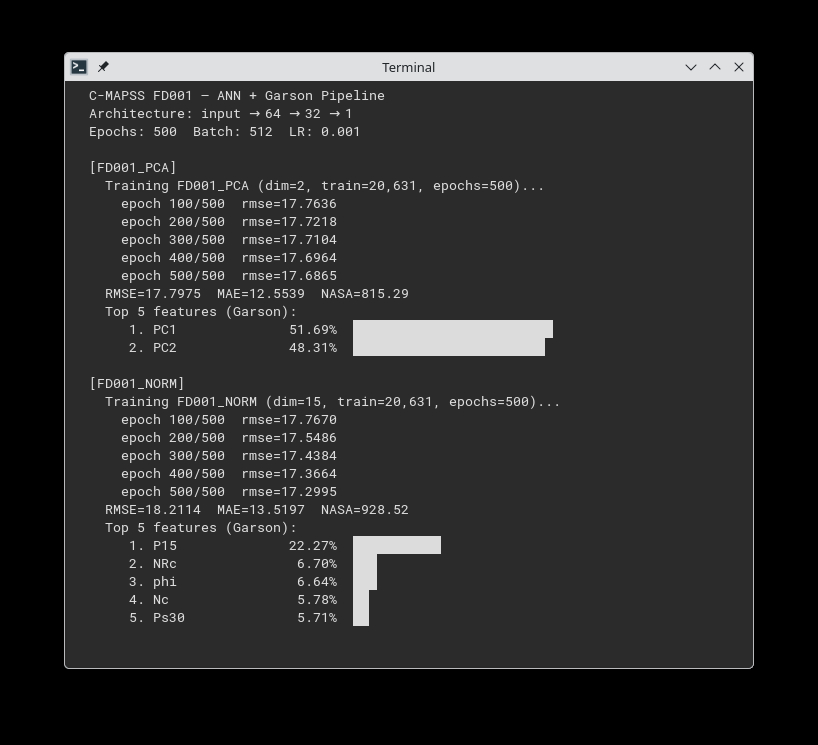
\includegraphics[width=0.80\textwidth]{images/python-10-fd001-term-01.png}
  \caption{Output terminal pelatihan --- FD001 PCA dan NORM, 500 epoch}
  \label{fig:ann_term1}
\end{figure}

\begin{figure}[H]
  \centering
  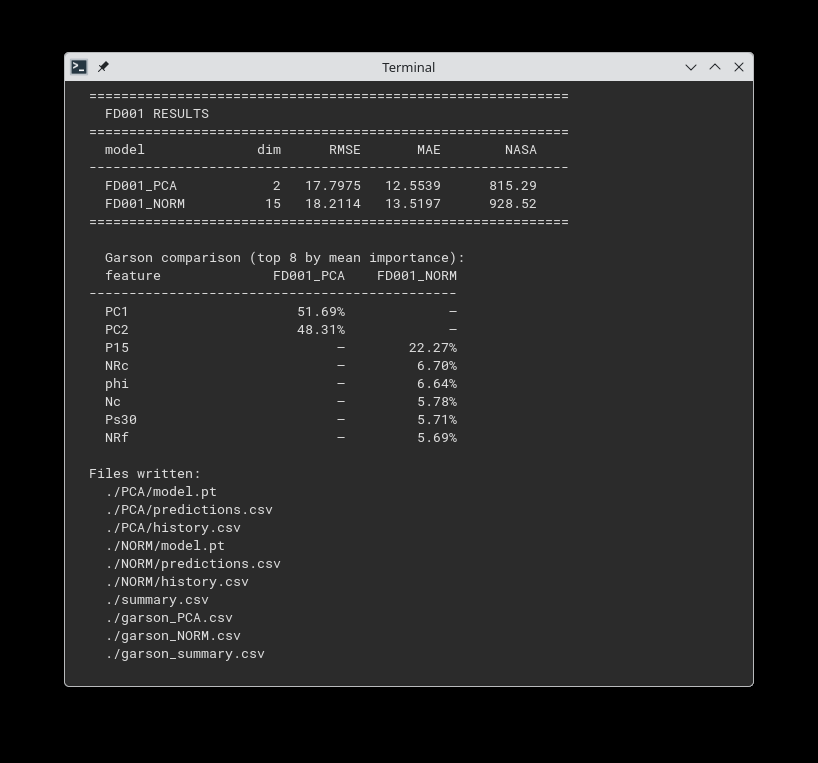
\includegraphics[width=0.80\textwidth]{images/python-10-fd001-term-02.png}
  \caption{Ringkasan hasil dan perbandingan Garson}
  \label{fig:ann_term2}
\end{figure}

\begin{table}[H]
\centering\small
\caption{Hasil perbandingan dua model FD001}
\label{tab:results}
\begin{tabular}{lcrrrr}
\toprule
Model & Input & Dim & RMSE & MAE & NASA Score \\
\midrule
\textbf{FD001\_PCA}  & PC1, PC2         & 2  &
  \textbf{17,7975} & \textbf{12,5539} & \textbf{815,29} \\
FD001\_NORM & 15 sensor & 15 &
  18,2114 & 13,5197 & 928,52 \\
\bottomrule
\end{tabular}
\end{table}

\subsection{Analisis Hasil}

Model PCA mengungguli NORM pada ketiga metrik. Hal ini menunjukkan bahwa
kompresi PCA (82,9\% varians dalam 2 komponen) efektif menghilangkan
\textit{noise} pada FD001 yang memiliki satu kondisi operasi dan satu mode
kerusakan sederhana. Model NORM dengan 15 fitur memiliki lebih banyak
parameter yang perlu dioptimalkan dalam jumlah epoch yang sama.

\textbf{NASA Score} --- Model PCA menghasilkan NASA Score lebih rendah
(815 vs 929), artinya lebih sedikit prediksi \textit{late} yang berbahaya.
Kurva penalti asimetris NASA Score ditunjukkan pada Gambar \ref{fig:nasa_score}.

\begin{figure}[H]
  \centering
  
\includegraphics[width=0.68\textwidth]{images/07_asymmetric_scoring_curve.png}
  \caption{Kurva penalti NASA Score --- prediksi \textit{late} ($d > 0$)
    dihukum lebih berat karena membahayakan keselamatan}
  \label{fig:nasa_score}
\end{figure}

% ══════════════════════════════════════════════════════════════════════════════
\section{Analisis Garson}

\subsection{Algoritma}

Algoritma Garson \cite{garson1991} menghitung kepentingan relatif fitur input
berdasarkan bobot jaringan terlatih. Untuk arsitektur dua lapisan tersembunyi
dengan matriks bobot $W_1\,(64{\times}n)$, $W_2\,(32{\times}64)$,
$W_3\,(1{\times}32)$:

\begin{align}
  q_1[i,j] &= \frac{|W_1[j,i]|}{\sum_k |W_1[j,k]|} &
  q_2[j,m] &= \frac{|W_2[m,j]|}{\sum_k |W_2[m,k]|} \\[4pt]
  r[i,m]   &= \sum_j q_1[i,j] \cdot q_2[j,m] &
  s[i]     &= \sum_m r[i,m] \cdot |W_3[m]| \\[4pt]
  \text{importance}[i] &= \frac{s[i]}{\sum_k s[k]}
\end{align}

Hasilnya adalah satu skor kepentingan per fitur, total 100\%.

\subsection{Hasil Model PCA}

\begin{table}[H]
\centering\small
\caption{Kepentingan fitur --- Model FD001\_PCA}
\label{tab:garson_pca}
\begin{tabular}{clr}
\toprule
Rank & Fitur & Kepentingan (\%) \\
\midrule
1 & PC1 & 51,69 \\
2 & PC2 & 48,31 \\
\bottomrule
\end{tabular}
\end{table}

Kedua komponen PCA hampir seimbang --- PC1 (kecepatan mesin, 52,4\% varians)
dan PC2 (kontras tekanan-kecepatan, 30,5\% varians) sama-sama penting untuk
prediksi RUL.

\subsection{Hasil Model NORM}

\begin{table}[H]
\centering\small
\caption{Kepentingan fitur --- Model FD001\_NORM (top 10)}
\label{tab:garson_norm}
\begin{tabular}{clr}
\toprule
Rank & Sensor & Kepentingan (\%) \\
\midrule
1  & P15     & 22,27 \\
2  & NRc     &  6,70 \\
3  & phi     &  6,64 \\
4  & Nc      &  5,78 \\
5  & Ps30    &  5,71 \\
6  & NRf     &  5,69 \\
7  & W32     &  5,65 \\
8  & T30     &  5,50 \\
9  & T50     &  5,47 \\
10 & P30     &  5,30 \\
\midrule
   & 5 sensor lainnya & 25,29 \\
\bottomrule
\end{tabular}
\end{table}

\subsection{Perbandingan Tiga Metode Seleksi Fitur}

\begin{table}[H]
\centering\small
\caption{Perbandingan kepentingan sensor: Pearson vs PCA vs Garson (FD001)}
\label{tab:three_method}
\begin{tabular}{lcccp{5cm}}
\toprule
Sensor & Pearson & PCA Loading & Garson & Interpretasi \\
\midrule
Ps30   & $-0{,}70$ & tinggi & sedang
  & Konsisten --- penting secara linear \\
T50    & $-0{,}68$ & tinggi & sedang
  & Konsisten --- penting secara linear \\
P30    & $+0{,}66$ & tinggi & sedang
  & Konsisten --- penting secara linear \\
\textbf{P15}
       & $-0{,}13$ & rendah & \textbf{22,27\%}
  & \textbf{Perbedaan} --- ANN menemukan sinyal non-linear \\
NRf    & $-0{,}56$ & sedang & rendah
  & Sebagian konsisten \\
\bottomrule
\end{tabular}
\end{table}

Temuan utama: sensor \textbf{P15} memiliki korelasi Pearson rendah
($-0{,}13$) dan kontribusi PCA rendah, namun Garson menetapkannya sebagai
fitur terpenting (22,27\%) pada model NORM. Hal ini mengindikasikan ANN
mampu mengeksploitasi hubungan non-linear yang tidak terdeteksi oleh metode
linear.

% ══════════════════════════════════════════════════════════════════════════════
\section{Kesimpulan}

\begin{enumerate}[noitemsep]
  \item \textbf{Enam sensor dieliminasi} (T2, P2, epr, farB, Nf\_dmd,
    PCNfR\_dmd) karena std $= 0$ --- tidak ada korelasi maupun variasi
    terhadap output RUL.

  \item \textbf{PCA menghasilkan 2 komponen} yang menjelaskan 82,9\% varians:
    PC1 merepresentasikan kecepatan mesin, PC2 merepresentasikan kontras
    tekanan-kecepatan.

  \item \textbf{Model PCA mengungguli NORM} pada FD001:
    RMSE 17,80 vs 18,21, NASA Score 815 vs 929.
    Kompresi PCA efektif untuk dataset dengan 1 kondisi operasi dan
    1 mode kerusakan.

  \item \textbf{Garson mengungkap sinyal non-linear}: sensor P15 ---
    Pearson rendah, PCA rendah --- terbukti paling penting menurut ANN
    (22,27\%), menunjukkan hubungan non-linear yang tidak terdeteksi
    metode linear.
\end{enumerate}

% ── References ────────────────────────────────────────────────────────────────
\begin{thebibliography}{9}
\bibitem{saxena2008}
  A. Saxena, K. Goebel, D. Simon, N. Eklund,
  ``Damage Propagation Modeling for Aircraft Engine Run-to-Failure Simulation,''
  \textit{Proc.\ 1st Int.\ Conf.\ Prognostics and Health Management (PHM08)},
  Denver, CO, 2008.

\bibitem{garson1991}
  G.D. Garson,
  ``Interpreting Neural Network Connection Weights,''
  \textit{AI Expert}, vol.~6, no.~4, pp.~46--51, 1991.
\end{thebibliography}

\end{document}
